%Needed for adobe reader to work
\pdfminorversion=4
\documentclass[compress]{beamer}
%for printing or having a crappy pdf reader backup
%\documentclass[handout]{beamer}
\mode<presentation>
\usetheme{Madrid}
\usecolortheme[RGB={128,128,128}]{structure}
\definecolor{my_gray}{RGB}{105,105,105}
\setbeamercolor{khumna}{fg=white,bg=my_gray}
%teal \usecolortheme[RGB={0,128,128}]{structure}
%\useoutertheme{miniframes}
\useinnertheme{default}
\usepackage{color}
\definecolor{Maroon}{RGB}{80,0,0}
\definecolor{BurntOrange}{RGB}{204,85,0}
\usepackage{setspace}
\usepackage{amsmath}
\usepackage{amsthm}
\usepackage{amsfonts}
\usepackage{amssymb}
\usepackage{verbatim}
\usepackage{array}
\usepackage{graphicx}
\usepackage{subfigure}
\usepackage{colortbl}
%\usepackage[retainorgcmds]{IEEEtrantools}
\usepackage{wrapfig}
\usepackage[figurename=,tablename=]{caption}
\usepackage{multirow}
\setbeamercolor{normal text}{fg=black}
\setbeamercovered{dynamic}
\beamertemplatetransparentcovereddynamicmedium
%\usepackage{chronology}
\setbeamertemplate{caption}[numbered]
\usepackage{colortbl}
\newcommand {\mathsym}[1]{{}}
\newcommand {\unicode}{{}}
\newcommand{\om}{\boldsymbol{\Omega}}
\newcommand{\etal}{{\it et al.\,}}
\newcommand{\vr}{\vec{r}}
\newcommand{\vo}{\vec{\Omega}}
\newcolumntype{L}{>{\centering\arraybackslash}m{3cm}}
\newcommand{\tcr}[1]{\textcolor{red}{#1}}
%Creating a norm command
\newcommand{\norm}[1]{\left\lVert#1\right\rVert}
%Allow page breaks within align
\allowdisplaybreaks
%Putting logo and banner in title and adding banner
\usepackage{textpos}
%Importing csv's directly
\usepackage{pgfplotstable}
%Code
\usepackage{listings}
\usepackage{epstopdf}
\usepackage{pdfpages}
\newlength \figwidth
\setlength \figwidth {0.5\textwidth}

\newcommand{\backupbegin}{
   \newcounter{finalframe}
   \setcounter{finalframe}{\value{framenumber}}
}
\newcommand{\backupend}{
   \setcounter{framenumber}{\value{finalframe}}
}

\addtobeamertemplate{frametitle}{}
{
	\begin{textblock*}{100mm}(0.85\textwidth,-1cm)
	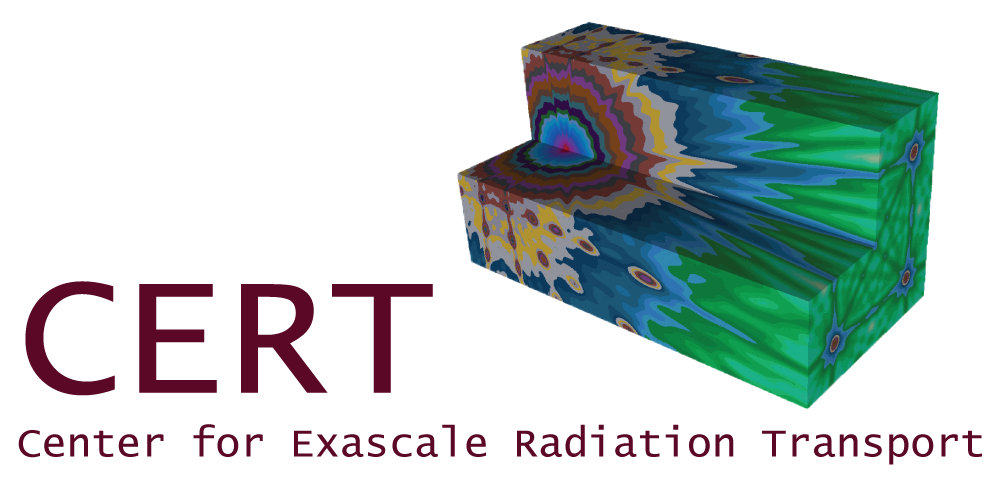
\includegraphics[height = 1cm,width=2cm]{figures/cert_logo_maroon.png}
	\end{textblock*}
}
\beamertemplatenavigationsymbolsempty



\begin{document}
%	

\title[Load Balancing]{An Update to Mesh Generation and Load Balancing in PDT}
\author[Ghaddar]{Tarek Ghaddar \\  Drs. Jean C. Ragusa \& Marvin L. Adams}
\institute[TAMU]{Texas A\&M University}
%\committee{Morel,Popov}{Dr. Jim Morel \\ Dr. Bojan Popov}
\date[May 2, 2017]

{
\setbeamertemplate{headline}{}
\begin{frame}
\vspace{-1.1cm}
	\begin{figure}[t]
		\centering
			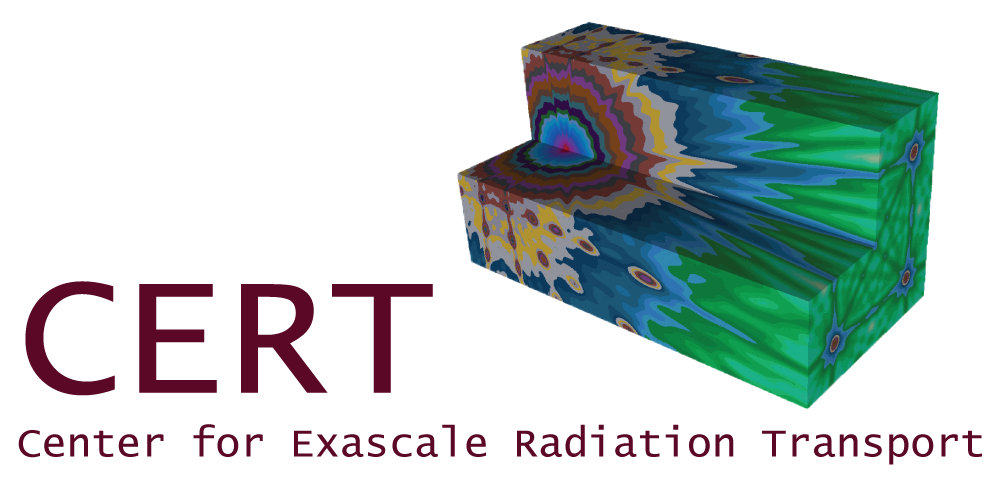
\includegraphics[width=.25\textwidth]{figures/cert_logo_maroon.png}
	\end{figure}
\vspace{-0.75cm}
\titlepage
\end{frame}
}

\setbeamertemplate{footline}
{

%\vspace{-0.1ex}
\begin{beamercolorbox}[wd=\textwidth,ht=3.5ex]{khumna}

\includegraphics[width = 0.95\textwidth]{figures/cert_banner.pdf}
	%\begin{textblock*}{10mm}(0.95\textwidth,10cm)
	\insertframenumber/\inserttotalframenumber
	%\end{textblock*}
\end{beamercolorbox}
%\begin{beamercolorbox}[wd=0.05\textwidth,ht=3.5ex]{khumna}

%\end{beamercolorbox}
}

\begin{frame}[t]\frametitle{Project Components and Integration}
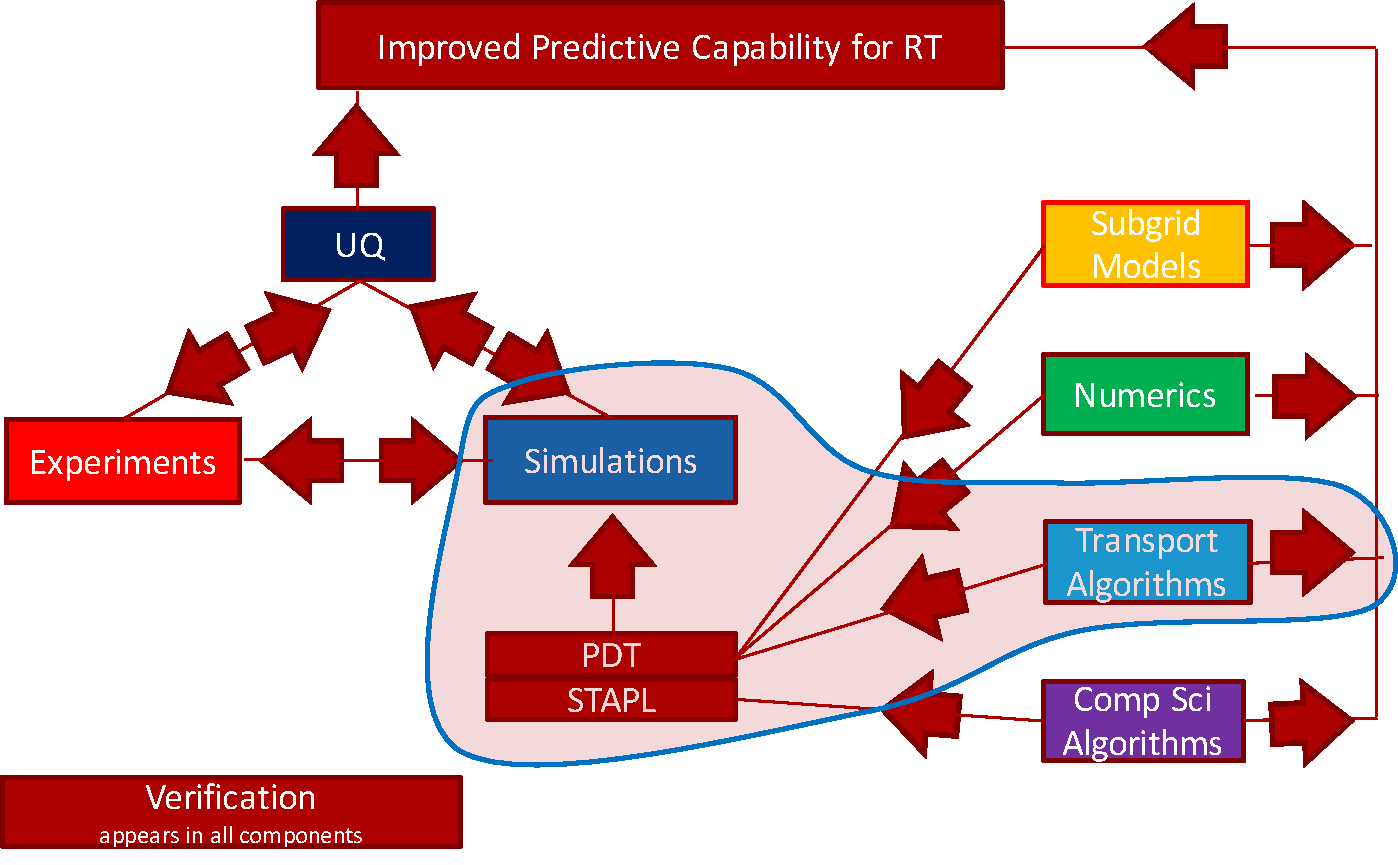
\includegraphics[scale = 0.45 ]{figures/Integration_Slide.pdf}
\end{frame}


\begin{frame}
\tableofcontents
\end{frame}

\section{Introduction}
%\subsection{}
\begin{frame}[t]\frametitle{Motivation}
	\begin{block}{}
	\begin{itemize}
		\item When running any massively parallel code, load balancing is a priority in order to achieve the best possible parallel efficiency.
		\item  A load balanced problem has an equal number of degrees of freedom per processor.
		\item Load balancing a logically Cartesian mesh is ``not difficult", as the user specifies the number of cells being used.
		\item In an unstructured mesh, the user cannot always specify the number of cells they want per processor, and obtaining a load balanced problem is more difficult.
		\item The goal is to implement a load balancing algorithm for unstructured meshes in PDT.
		\item Our problem is unique because we need our cellsets to be convex (bricks for now) because bricks are provably optimal.
	\end{itemize}
	\end{block}
\end{frame}

\begin{frame}[t]\frametitle{The Triangle Mesh Generator}
	\begin{block}{}
	\begin{itemize}
		\item Unstructured meshes in PDT are generated in 2D using the Triangle Mesh Generator.
		\item These can be extruded to create 3D meshes.
		\item Fixes by Daryl Hawkins within the Triangle source code have lead to much more stable mesh generation for complex geometries.
	\end{itemize}	
	\end{block}
	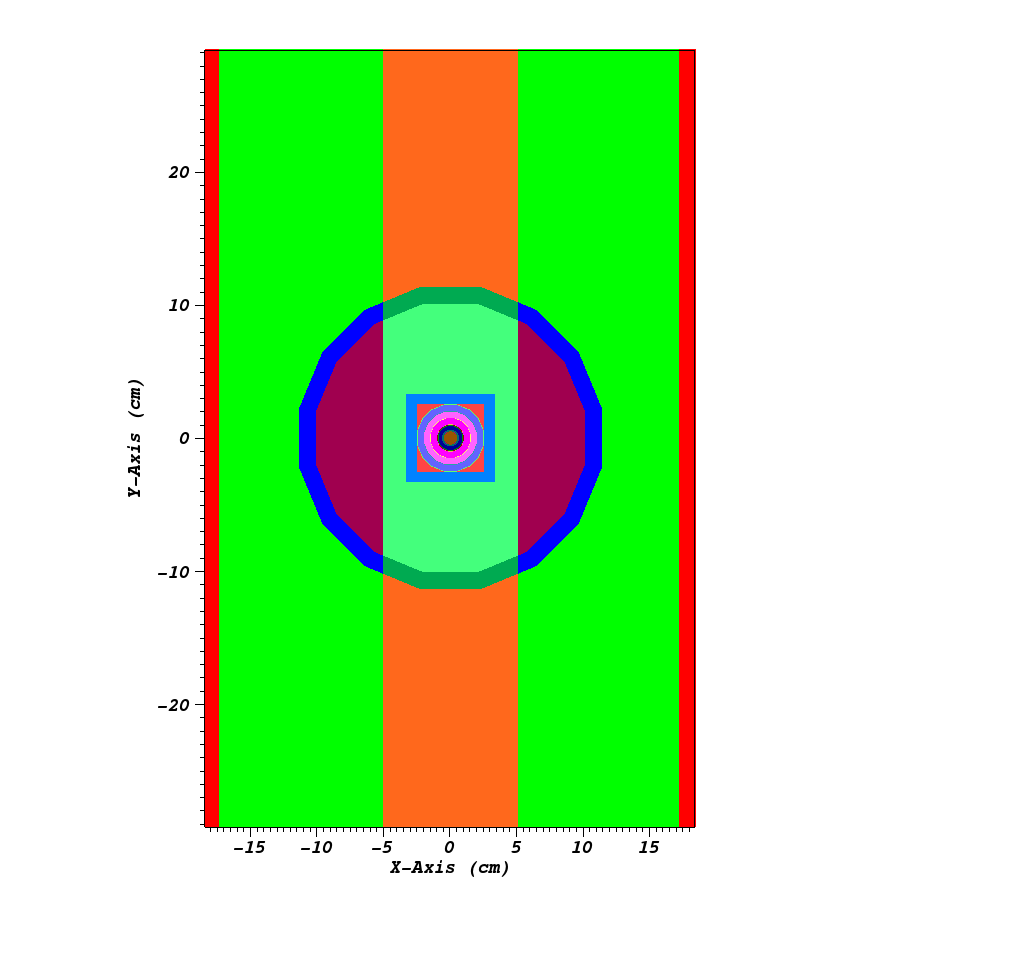
\includegraphics[scale = 0.15]{figures/IM12DPoly.png}
	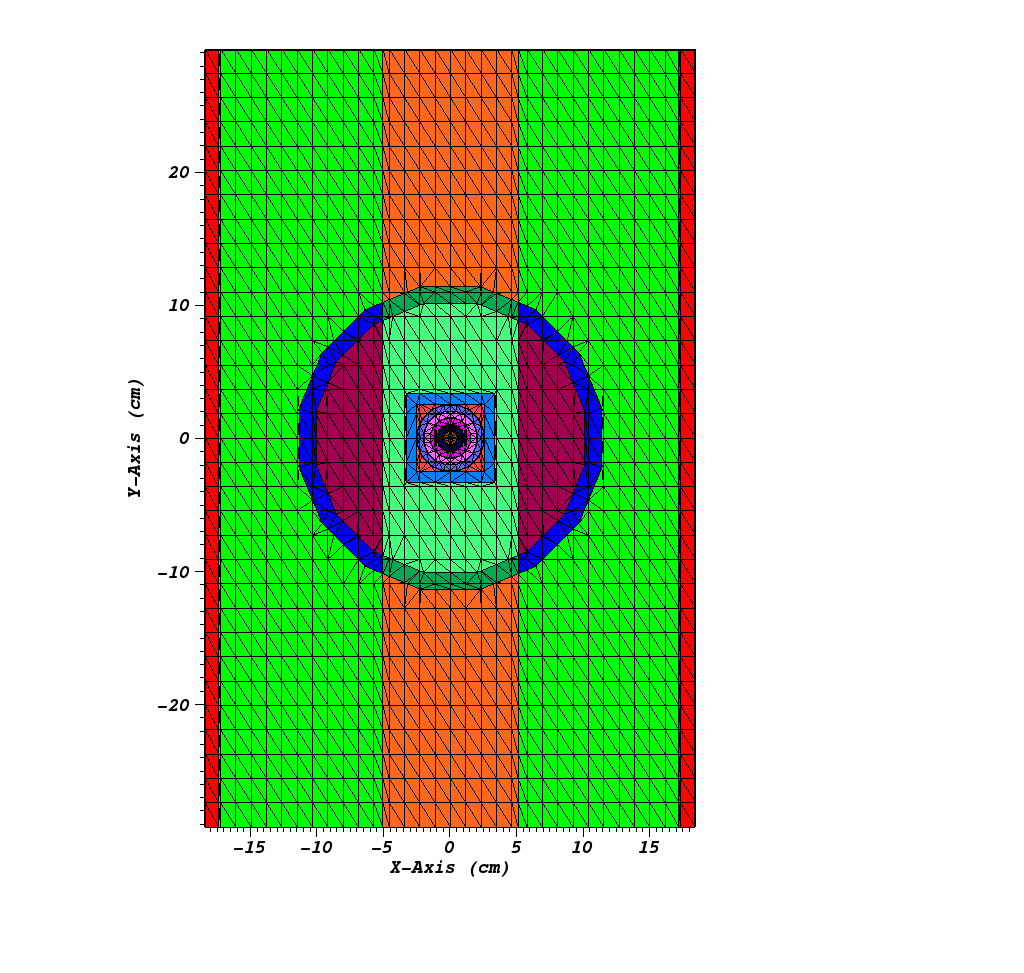
\includegraphics[scale = 0.15]{figures/IM12DMesh.png}
\end{frame}

\section{Load Balance Algorithm}
%\subsection{}

\begin{frame}[t]\frametitle{Partitioning for an Unstructured Mesh}
\begin{block}{}
	\begin{itemize}
	\item The user inputs coordinates for cut lines in the X and Y directions.
	\item The cut lines will determine the number of ``subsets" the problem is partitioned into.
	\item Optimizing the location of these cut lines is the basis of the load balancing algorithm.
	\item A ``subset" is a rectangular unit that is formed by intersecting cut lines.
	\end{itemize}
\end{block}
\end{frame}

\begin{frame}[t]\frametitle{The Subset}
\centering
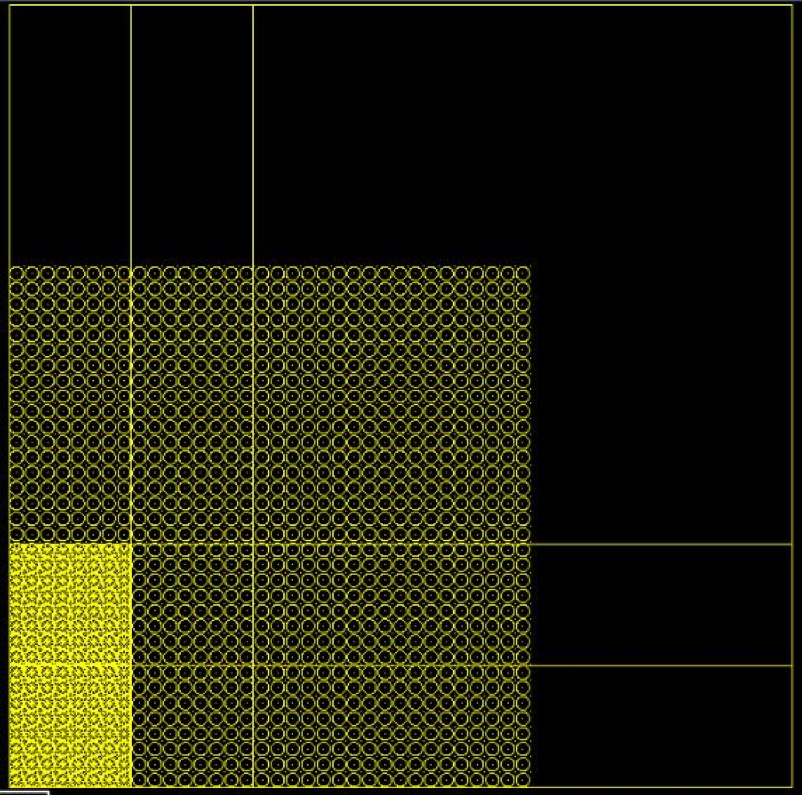
\includegraphics[width = 12 cm, height = 7 cm ]{figures/subsetlattice.png}
\end{frame}

\begin{frame}[t]\frametitle{ Goal and Definitions}
	\begin{block}{}
	
		\begin{itemize}
			\item \textbf{Goal:} Obtain an equal number of cells per processor, which for our purposes means an equal number of cells per subset.
			\item Achieved by optimizing the location of $X_i$ and $Y_j$, the location of the cut lines.
			%\item We define the load balance metric, $f$.
			\item \textbf{Define}:
			\begin{itemize}
			\item $N_{ij}$: The number of cells  in subset ${i,j}$
			%\item Cut Lines: $X_i, Y_j$, $1 <= i <= I-1$, $1 <= j <= J-1$
			\item $f =\frac{\underset{ij}{\text{max}}(N_{ij})}{\frac{N_{tot}}{I\cdot J}}$
			\item $f_I = \underset{i}{\text{max}}[\sum_{j} N_{ij}]/\frac{N_{tot}}{I}$
			\item $f_J = \underset{j}{\text{max}}[\sum_{i} N_{ij}]/\frac{N_{tot}}{J}$
			\item $f_{J_i} = \text{max}[N_{ij}]_i/\frac{\sum_{j}N_{ij}}{J}$
			\end{itemize}
		\end{itemize}
	\end{block}
\end{frame}

\begin{frame}[t]\frametitle{Original Load Balancing Algorithm}
\vspace{-0.5 cm}
\begin{block}{}
\lstinputlisting[language = C++, basicstyle = \footnotesize]{loadbalance.cc}
\end{block}
\end{frame}

\begin{frame}[t]\frametitle{Why a new algorithm?}
\centering
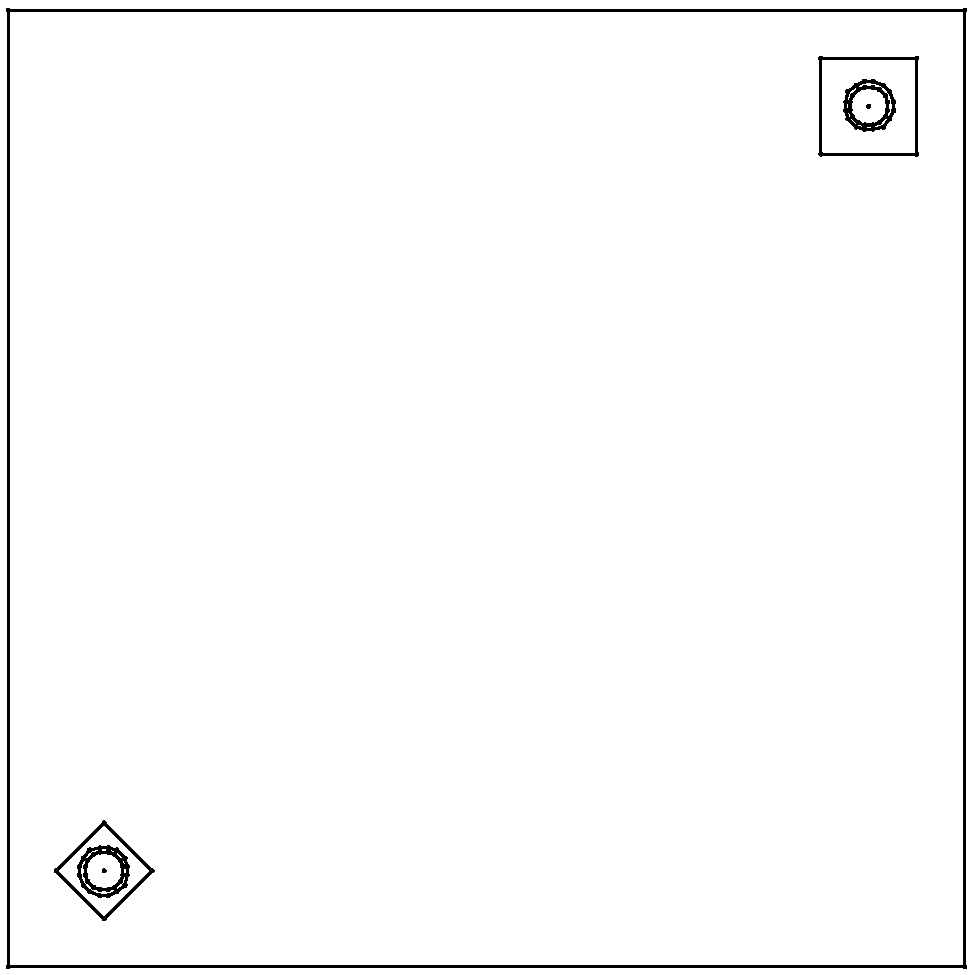
\includegraphics[scale = 0.3]{figures/unbalanced_lattice-eps-converted-to.pdf}
\begin{block}{}
\begin{itemize}
\item Limited effectiveness if we don't move more cut lines into BOTH features.
\item We allow one dimension's cut lines to be moved by row/column rather than cut all the way through the problem. 
\end{itemize}
\end{block}
\end{frame}

\begin{frame}[t]\frametitle{Challenges}
\begin{block}{}
\begin{itemize}
\item Altering and tinkering with the algorithm is not difficult.
\item However, a completely new stitching algorithm had to be written.
\item The old stitching algorithm assumed one neighboring subset to the north, south, east and west.
\item We now have an arbitrary number of neighbors in the north/south or east/west directions.
\end{itemize}
\end{block}
\end{frame}

\begin{frame}[t]\frametitle{Load Balancing By Dimension Algorithm}
\vspace{-0.5 cm}
\begin{block}{}
\lstinputlisting[language = C++, basicstyle = \footnotesize]{load_balance_by_dimension.cc}
\end{block}
\end{frame}

\begin{frame}[t]\frametitle{Redistribution Function}
\centering
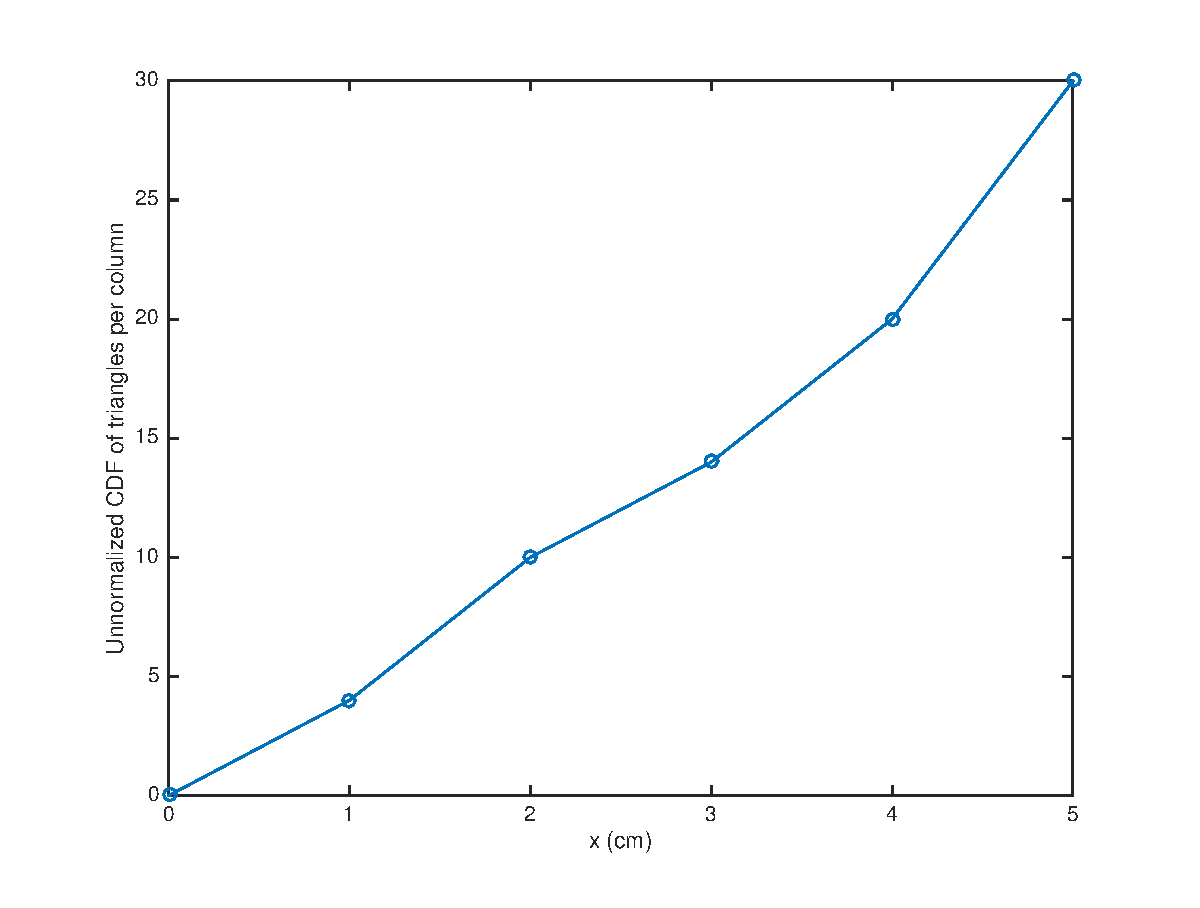
\includegraphics[scale = 0.5]{figures/before_redistribute.eps}
\end{frame}

\begin{frame}[t]\frametitle{Redistribution Function}
\centering
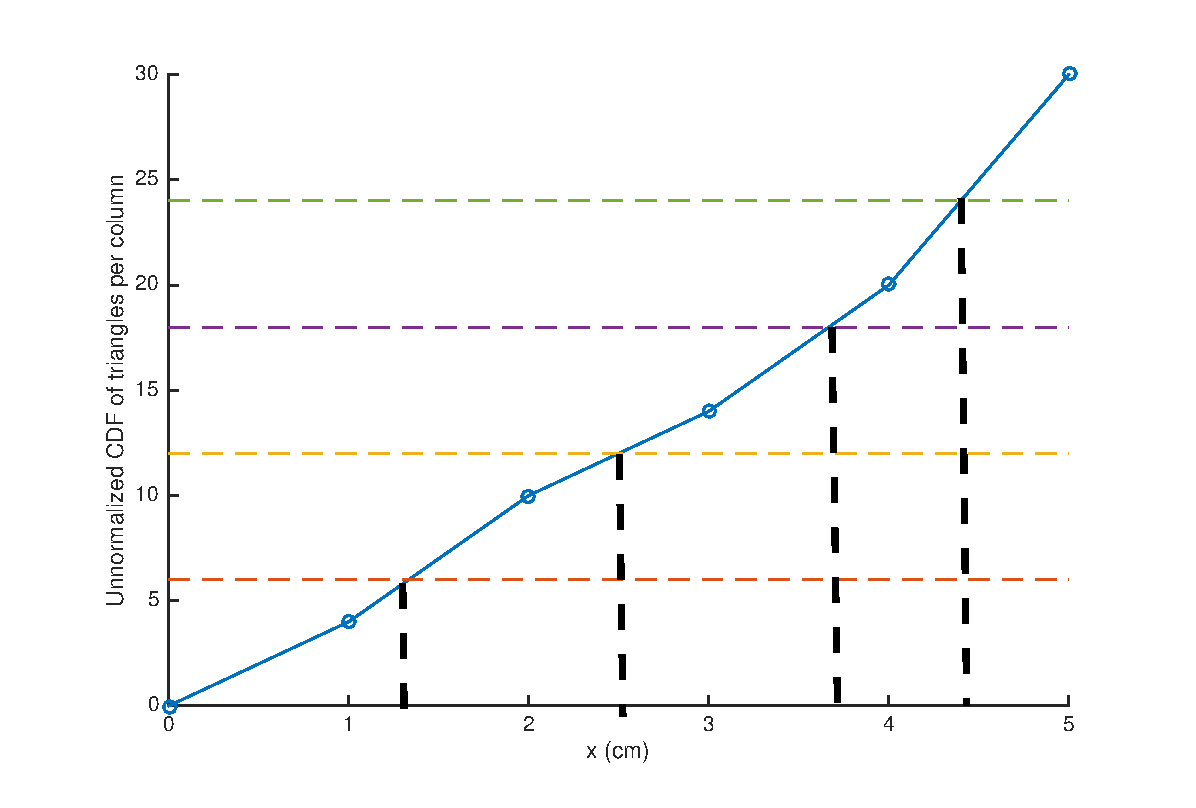
\includegraphics[scale = 0.5]{figures/after_redistribute.eps}
\end{frame}

\section{Load Balancing Results}
%\subsection{}
\begin{frame}[t]\frametitle{Load Balancing Results}
\begin{block}{}
\begin{itemize}
	\item Two test cases were used to study the behavior of both load balancing algorithms.
	\item For each test case, 162 inputs were constructed by varying:
		\begin{itemize}
		\item The number of subsets
		\item The spatial resolution of the mesh (maximum triangle area).
		\end{itemize}
\end{itemize}
\end{block}
\end{frame}

\begin{frame}[t]\frametitle{Test Case 1}
\centering
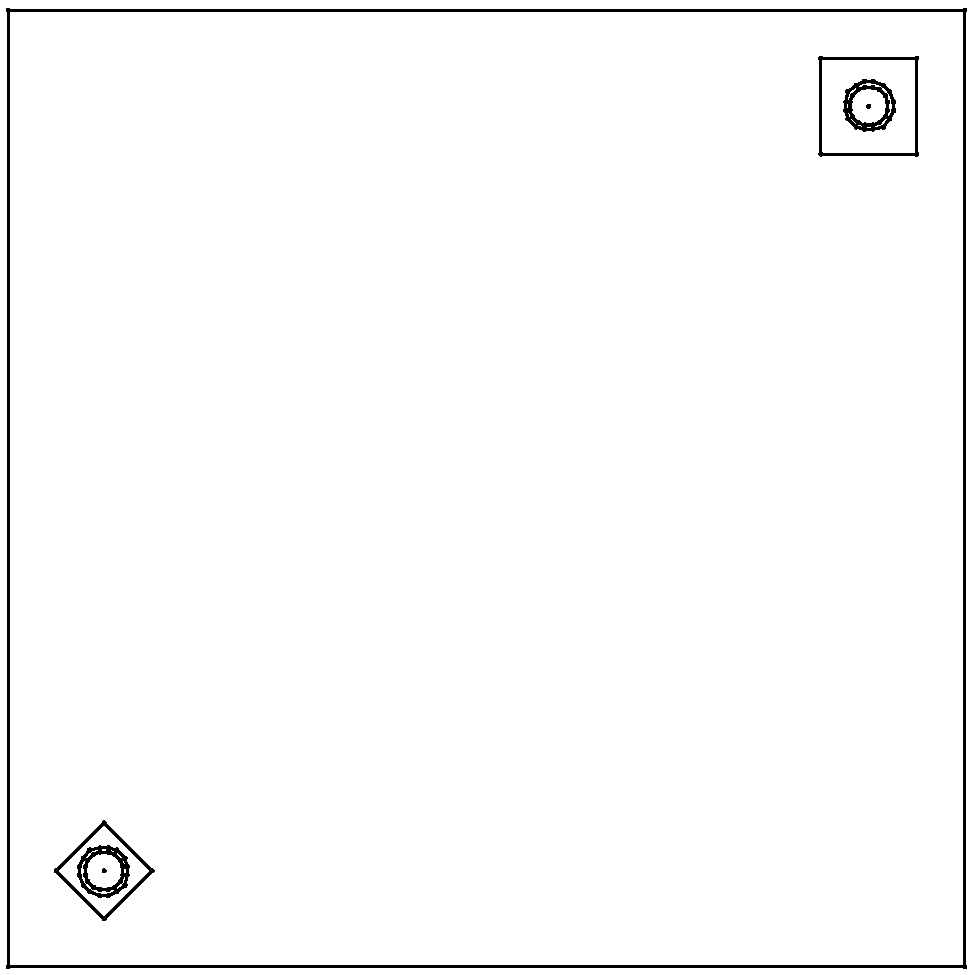
\includegraphics[scale = 0.4]{figures/unbalanced_lattice-eps-converted-to.pdf}
\end{frame}


%Tabulate iterations
\begin{frame}[t]\frametitle{Test Case 1 - Original Load Balancing Method}
\begin{table}[H]
\tiny
\centering
\caption{The best metric behavior of the first test case after \textbf{10 load balancing iterations}.} 
\begin{tabular}{rrrrrllrll}
\hline
 Area & 2x2 &3x3 & 4x4 & 5x5 & 6x6 & 7x7 &8x8 & 9x9 & 10x10 \\ 
\hline
 Coarse   & 1.94872 & 1.59813 & 3.36842 & 2.0979  & 2.27848 & 2.67760 & 2.53465 & 2.80519 & 3.05344 \\
  1.8  & 1.2636  & 1.7963  & 2.61017 & 2.25049 & 2.22889 & 2.77358 & 3.61199 & 3.25628 & 3.46457 \\
  1.6  & 1.28    & 1.73805 & 2.4186  & 3.42205 & 2.33094 & 2.52144 & 3.53821 & 3.31132 & 3.39506 \\
  1.4  & 1.25913 & 1.63776 & 2.22819 & 2.76946 & 2.37232 & 2.64418 & 3.45946 & 3.52685 & 3.60360 \\
  1.2  & 1.21557 & 1.60763 & 2.13982 & 2.75424 & 1.97260 & 2.50150 & 3.22238 & 3.87560 & 3.92670 \\
  1    & 1.16754 & 1.50773 & 1.99222 & 2.63505 & 1.78302 & 2.23291 & 2.53968 & 3.67303 & \textbf{\cellcolor{blue!25}4.32173} \\
  0.8  & 1.1486  & 1.51935 & 1.70576 & 2.37342 & 2.91692 & 1.94566 & 2.56263 & 2.62348 & crash   \\
  0.6  & 1.10711 & 1.40017 & 1.64962 & 1.98312 & 2.29787 & 1.69898 & 1.88852 & 2.40594 & 3.09917 \\
  0.4  & 1.07855 & 1.26344 & 1.57126 & 1.65698 & 2.02992 & 2.19854 & 1.73657 & 1.75030 & 2.06311 \\
  0.2  & 1.04278 & 1.12703 & 1.255   & 1.40941 & 1.59606 & 1.76163 & 1.29236 & crash   & 1.44558 \\
  0.1  & 1.01421 & 1.06717 & 1.12843 & 1.21254 & 1.27065 & crash   & 1.48006 & crash   & 1.24494 \\
  0.08 & 1.01331 & 1.03474 & 1.04114 & 1.14352 & crash   & crash   & 1.33911 & crash   & 1.17602 \\
  0.06 & 1.01816 & 1.02969 & 1.0604  & 1.08645 & crash   & 1.14368 & 1.23391 & crash   & 1.06347 \\
  0.05 & 1.00671 & 1.02257 & 1.05096 & 1.07697 & crash   & 1.08246 & 1.19871 & crash   & 1.08662 \\
  0.04 & 1.00584 & 1.01853 & 1.00844 & 1.02842 & crash   & 1.05551 & 1.09949 & crash   & 1.10996 \\
  0.03 & 1.00455 & 1.01347 & 1.03663 & 1.06479 & crash   & crash   & 1.06606 & crash   & 1.03406 \\
  0.02 & 1.00414 & 1.00661 & 1.00282 & 1.00369 & 1.02310 & crash   & 1.0028  & 1.04513 & 1.04855 \\
  0.01 & 1.0025  & 1.0078  & 1.01399 & \textbf{\cellcolor{blue!25}1.00038} & 1.01219 & 1.01801 & 1.00265 & 1.03554 & 1.00967 \\
\hline
\end{tabular}
\end{table}
\end{frame}


\begin{frame}[t]\frametitle{Test Case 1 - Load Balancing By Dimension}
\begin{table}[H]
\tiny
\centering
\caption{The best metric behavior of the first test case after \textbf{10 load balancing by dimension iterations}.} 
 \begin{tabular}{rrrrrllrlr}
 \hline
  Area & 2x2 &3x3 & 4x4 & 5x5 & 6x6 & 7x7 &8x8 & 9x9 & 10x10 \\ 
\hline
 Coarse    & 1.85366 & 1.20536 & 1.47518 & 1.39752 & 1.26000 & 1.36744 & 1.42751 & 1.62542 & 1.63934 \\
  1.8  & 1.075   & 1.38996 & 1.16364 & 1.47849 & 1.33539 & 1.43673 & 1.62712 & 1.69693 & 1.54639 \\
  1.6  & 1.09427 & 1.17033 & 1.20548 & 1.47569 & 1.18919 & 1.61862 & 1.60894 & 1.64676 & 1.9347  \\
  1.4  & 1.0785  & 1.0623  & 2.04361 & 1.25369 & 1.34370 & 1.74521 & 1.50196 & 1.74194 & \textbf{\cellcolor{blue!25}2.25166} \\
  1.2  & 1.06466 & 1.16594 & 1.84155 & 1.24481 & 1.43795 & 1.31624 & 1.67221 & 1.61105 & 1.68651 \\
  1    & 1.02767 & 1.0814  & 1.66581 & 1.16686 & 1.32857 & 1.21260 & 1.30879 & 1.73394 & 1.69651 \\
  0.8  & 1.00539 & 1.07843 & 1.24239 & 1.21888 & 1.26000 & 1.32965 & 1.62025 & 1.40503 & 1.6791  \\
  0.6  & 1.00916 & 1.08    & 1.08826 & 1.19048 & 1.14241 & 1.22023 & 1.23839 & 1.53759 & 1.44509 \\
  0.4  & 1.07855 & 1.09059 & 1.0405  & 1.21576 & 1.16923 & 1.16009 & 1.12629 & 1.38937 & 1.47929 \\
  0.2  & 1.04278 & 1.04741 & 1.07522 & 1.09865 & 1.06383 & 1.10162 & 1.14798 & crash   & 1.19151 \\
  0.1  & 1.01421 & 1.06717 & 1.04461 & 1.04716 & 1.07173 & crash   & 1.04762 & crash   & 1.13249 \\
  0.08 & 1.01331 & 1.03474 & 1.04114 & 1.04061 & crash   & crash   & 1.08798 & crash   & 1.08844 \\
  0.06 & 1.01816 & 1.02969 & 1.0604  & 1.08645 & crash   & 1.07748 & 1.07019 & crash   & 1.06347 \\
  0.05 & 1.00671 & 1.02257 & 1.05096 & 1.07697 & crash   & 1.08246 & 1.08371 & crash   & 1.08662 \\
  0.04 & 1.00584 & 1.01853 & 1.00844 & 1.02842 & crash   & 1.05551 & 1.09949 & crash   & 1.0496  \\
  0.03 & 1.00455 & 1.01347 & 1.03663 & 1.06479 & crash   & crash   & 1.06606 & crash   & 1.03406 \\
  0.02 & 1.00414 & 1.00661 & 1.00282 & 1.00369 & 1.02310 & crash   & 1.0028  & 1.04513 & 1.04855 \\
  0.01 & 1.0025  & 1.0078  & 1.01399 & \textbf{\cellcolor{blue!25}1.00038} & 1.01219 & 1.01801 & 1.00265 & 1.03554 & 1.00967 \\
\hline
\end{tabular}
 \end{table}
\end{frame}

%BAD RESULTS
\begin{frame}[t]\frametitle{Test Case 1 - Original Load Balancing Method}
\begin{table}[H]
\tiny
\centering
\caption{The best metric behavior of the first test case after \textbf{10 load balancing iterations}.} 
\begin{tabular}{rrrrrrrrrr}
\hline
  Area & 2x2 &3x3 & 4x4 & 5x5 & 6x6 & 7x7 &8x8 & 9x9 & 10x10 \\ 
\hline
 Coarse& 1.949 & 1.598 & 3.368 & 2.098 & 2.278 & 2.678 & 2.535 & 2.805 & 3.053 \\
 1.8 &1.458 & 1.940 & 2.449 & 2.590 & 2.980 & 3.441 & 2.957 & 4.657 & 3.434 \\
 1.6 & 1.423 & 1.949 & 2.427 & 2.411 & 3.004 & 3.053 & 3.579 & 4.107 & 4.105 \\
 1.4 & 1.316 & 1.871 & 2.654 & 3.130 & 2.451 & 3.030 & 3.473 & 4.040 & 3.898 \\
 1.2 & 1.298 & 1.765 & 2.462 & 2.656 & 2.592 & 3.178 & 3.144 & 4.282 & \textbf{\cellcolor{blue!25}4.683} \\
 1 & 1.348 & 1.638 & 2.260 & 2.327 & 2.347 & 3.013 & 3.357 & 3.841 & 4.245 \\
 0.8 & 1.257 & 1.513 & 2.017 & 2.792 & 2.018 & 2.617 & 2.884 & 3.423 & 3.629 \\
 0.6 & 1.142 & 1.452 & 1.788 & 2.408 & 2.332 & 2.092 & 2.669 & 2.874 & 3.629 \\
 0.4 & 1.095 & 1.353 & 1.449 & 1.872 & 2.397 & 1.836 & 2.153 & 2.351 & 2.262 \\
 0.2 & 1.046 & 1.136 & 1.336 & 1.545 & 1.648 & 2.049 & 1.678 & 1.790 & 1.714 \\
 0.1 & 1.020 & 1.043 & 1.109 & 1.170 & 1.287 & 1.357 & 1.297 & 1.409 & 1.221 \\
 0.08 & 1.011 & 1.029 & 1.094 & 1.190 & 1.209 & 1.290 & 1.268 & 1.318 & 1.381 \\
 0.06 & 1.005 & 1.031 & 1.037 & 1.105 & 1.087 & 1.189 & 1.177 & 1.283 & 1.068 \\
 0.05 & 1.021 & 1.022 & 1.058 & 1.092 & 1.079 & 1.115 & 1.157 & 1.218 & 1.176 \\
 0.04 & 1.004 & 1.013 & \textbf{\cellcolor{blue!25}1.002} & 1.061 & 1.074 & 1.073 & 1.158 & 1.171 & 1.171 \\
 0.03 & 1.003 & 1.016 & 1.021 & 1.050 & 1.065 & 1.048 & 1.928 & 1.132 & 1.041 \\
 0.02 & 1.004 & 1.008 & 1.010 & 1.034 & 1.024 & 1.028 & 1.574 & 1.075 & 1.094 \\
 0.01& 1.003 & 1.010 & 1.008 & 1.009 & 1.039 & 1.018 & 1.276 & 1.043 & 1.022 \\
\hline
\end{tabular}
\end{table}
\end{frame}

\begin{frame}[t]\frametitle{Test Case 1 - Load Balancing By Dimension}
\begin{table}[H]
\tiny
\centering
\caption{The best metric behavior of the first test case after \textbf{10 load balancing by dimension iterations}.} 
\begin{tabular}{rrrrrrrrrr}
 \hline
 Area & 2x2 &3x3 & 4x4 & 5x5 & 6x6 & 7x7 &8x8 & 9x9 & 10x10 \\ 
\hline
 Coarse & 1.854 & 1.205 & 1.475 & 1.398 & 1.260 & 1.367 & 1.428 & 1.625 & 1.639 \\
  1.800 & 1.079 & 1.392 & 1.523 & 1.722 & 2.036 & 2.315 & 2.421 & 3.962 & 3.587 \\
  1.600 & 1.044 & 1.704 & 1.536 & 1.566 & 1.791 & 2.126 & 2.492 & 3.417 & 3.807 \\
  1.400 & 1.073 & 1.152 & 1.509 & 1.756 & 1.811 & 2.183 & 2.475 & 2.911 & \textbf{\cellcolor{blue!25}3.974} \\
  1.200 & 1.037 & 1.125 & 1.515 & 1.718 & 1.972 & 2.611 & 2.628 & 3.816 & 3.205 \\
  1.000 & 1.047 & 1.209 & 1.180 & 1.763 & 1.494 & 1.928 & 2.564 & 3.744 & 3.953 \\
  0.800 & 1.077 & 1.193 & 1.246 & 1.343 & 1.417 & 2.949 & 2.411 & 3.560 & 3.629 \\
  0.600 & 1.066 & 1.112 & 1.388 & 1.455 & 1.521 & 1.837 & 1.769 & 2.586 & 3.381 \\
  0.400 & 1.095 & 1.032 & 1.145 & 1.221 & 1.479 & 1.355 & 1.554 & 2.038 & 1.838 \\
  0.200 & 1.046 & 1.049 & 1.075 & 1.149 & 1.173 & 1.174 & 1.210 & 1.251 & 1.571 \\
  0.100 & 1.020 & 1.043 & 1.023 & 1.071 & 1.103 & 1.138 & 1.129 & 1.091 & 1.205 \\
  0.080 & 1.011 & 1.029 & 1.094 & 1.072 & 1.076 & 1.097 & 1.068 & 1.071 & 1.213 \\
  0.060 & 1.005 & 1.031 & 1.037 & 1.016 & 1.087 & 1.096 & 1.093 & 1.095 & 1.068 \\
  0.050 & 1.021 & 1.022 & 1.058 & 1.092 & 1.079 & 1.062 & 1.090 & 1.075 & 1.088 \\
  0.040 & 1.004 & 1.013 & 1\textbf{\cellcolor{blue!25}.002} & 1.061 & 1.074 & 1.073 & 1.067 & 1.090 & 1.100 \\
  0.030 & 1.003 & 1.016 & 1.021 & 1.050 & 1.065 & 1.048 & 1.038 & 1.061 & 1.041 \\
  0.020 & 1.004 & 1.008 & 1.010 & 1.034 & 1.024 & 1.028 & 1.058 & 1.075 & 1.094 \\
  0.010 & 1.003 & 1.010 & 1.008 & 1.009 & 1.039 & 1.018 & 1.054 & 1.043 & 1.022 \\
\hline
\end{tabular}
\end{table}
\end{frame}

\begin{frame}[t]\frametitle{Test Case 2}
\centering
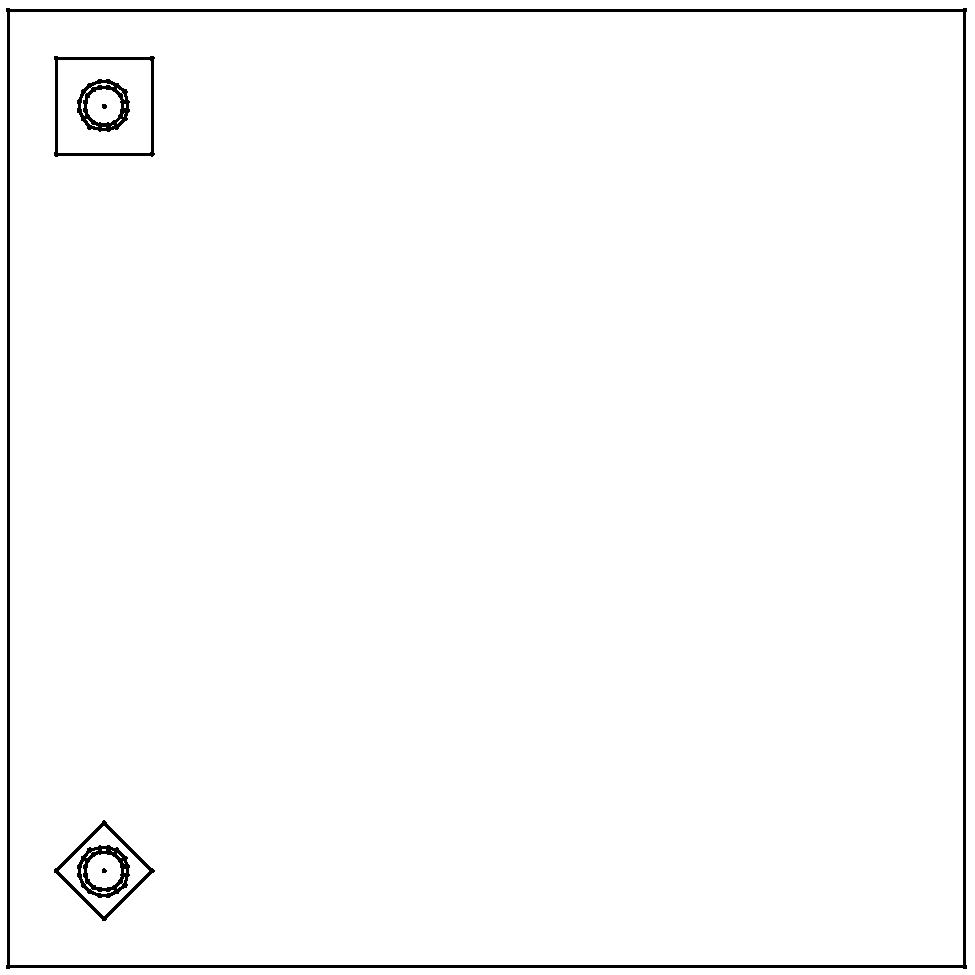
\includegraphics[scale = 0.4]{figures/unbalanced_pins_same_side-eps-converted-to.pdf}
\end{frame}

\begin{frame}[t]\frametitle{Test Case 2 - Original Load Balancing Method}
\begin{table}[H]
\centering
\tiny
\caption{The best metric behavior of the second test case after \textbf{10 load balancing iterations}.} 
\begin{tabular}{rrrrllllll}
\hline
  Area & 2x2 &3x3 & 4x4 & 5x5 & 6x6 & 7x7 &8x8 & 9x9 & 10x10 \\ 
\hline
 Coarse    & 1.85366 & 1.36134 & 1.76471 & 1.47929 & 1.74194 & 1.59535 & 1.79200 & 1.82022 & 1.92308 \\
  1.8  & 1.05051 & 1.46429 & 1.91617 & 1.79245 & 1.67742 & 2.03109 & 2.46154 & 2.40000 & crash   \\
  1.6  & 1.12334 & 1.36667 & 1.52113 & 1.51246 & 1.74000 & 1.88160 & 2.41860 & 2.42120 & crash   \\
  1.4  & 1.0798  & 1.36224 & 1.50405 & 1.68971 & 1.78882 & 1.81762 & 2.02590 & 2.50633 & 2.90621 \\
  1.2  & 1.08982 & 1.31642 & 1.53392 & 1.83206 & 1.72197 & 1.77437 & 2.18947 & 1.96364 & 2.55814 \\
  1    & 1.06144 & 1.22093 & 1.7405  & 1.58269 & 1.57241 & 1.90522 & 2.05686 & 2.52561 & 2.76890 \\
  0.8  & 1.03786 & 1.29399 & 1.57676 & crash   & 1.81635 & 1.63333 & 1.94892 & 2.07897 & crash   \\
  0.6  & 1.02013 & 1.24191 & 1.45577 & 1.62018 & 1.89176 & 1.54088 & 1.68019 & 2.09201 & 2.42057 \\
  0.4  & 1.08708 & 1.15836 & 1.35356 & 1.53151 & 1.49309 & 1.62142 & crash   & 1.84091 & 2.06311 \\
  0.2  & 1.04385 & 1.13315 & 1.14008 & 1.30224 & 1.41835 & 1.46784 & crash   & crash   & 1.44558 \\
  0.1  & 1.01452 & 1.06382 & 1.08479 & 1.21254 & 1.27404 & crash   & 1.17664 & crash   & 1.24494 \\
  0.08 & 1.00326 & 1.03738 & 1.07394 & 1.14352 & crash   & crash   & 1.33779 & crash   & 1.17602 \\
  0.06 & 1.01328 & 1.03467 & 1.0608  & 1.09088 & crash   & 1.15676 & 1.23391 & crash   & 1.06356 \\
  0.05 & 1.00719 & 1.02003 & 1.04326 & 1.08069 & crash   & 1.09384 & 1.19785 & crash   & 1.08696 \\
  0.04 & 1.00526 & 1.01942 & 1.00869 & 1.03234 & crash   & 1.04483 & 1.09539 & crash   & 1.10996 \\
  0.03 & 1.00577 & 1.011   & 1.00672 & 1.03871 & 1.08489 & crash   & 1.08146 & crash   & 1.03406 \\
  0.02 & 1.00403 & 1.00874 & 1.00382 & 1.01427 & 1.02385 & crash   & 1.00326 & 1.04696 & 1.04855 \\
  0.01 & 1.00262 & 1.00788 & 1.01374 & 1.00126 & 1.01320 & 1.01755 & 1.00276 & 1.03491 & 1.00970 \\
\hline
\end{tabular}
\end{table}
\end{frame}

\begin{frame}[t]\frametitle{Test Case 2 - Load Balancing By Dimension}
\begin{table}[H]
\tiny
\centering
\caption{The best metric behavior of the second test case after \textbf{10 load balancing by dimension iterations}.} 
\begin{tabular}{rrrrrllrlr}
\hline
 Coarse    & 1.85366 & 1.13445 & 1.67164 & 1.32353 & 1.65306 & 1.51770 & 1.54217 & 1.40138 & 1.51976 \\
  1.8  & 1.05051 & 1.08271 & 1.38346 & 1.33556 & 1.29836 & 1.42488 & 1.45897 & 1.59944 & 1.69014 \\
  1.6  & 1.02642 & 1.19355 & 1.15697 & 1.30769 & 1.43385 & 1.39403 & 1.38753 & 1.59270 & 1.76322 \\
  1.4  & 1.0798  & 1.1068  & 1.2     & 1.34707 & 1.73077 & 1.45283 & 1.6     & 1.81184 & 1.61663 \\
  1.2  & 1.08982 & 1.12848 & 1.25346 & 1.28205 & 1.25301 & 1.77032 & 1.48263 & 1.70926 & 1.64271 \\
  1    & 1.06144 & 1.0616  & 1.1673  & 1.37699 & 1.24444 & 1.67726 & 1.48211 & 1.50309 & 1.64103 \\
  0.8  & 1.03786 & 1.06441 & 1.26716 & 1.31579 & 1.37626 & 1.40286 & 1.44696 & 1.40870 & 1.64076 \\
  0.6  & 1.02013 & 1.09756 & 1.17936 & 1.23865 & 1.16505 & 1.28419 & 1.45344 & 1.29106 & 1.32013 \\
  0.4  & 1.08708 & 1.04824 & 1.08222 & 1.06178 & 1.23995 & 1.15526 & 1.10851 & 1.41856 & 1.46396 \\
  0.2  & 1.04385 & 1.06826 & 1.03802 & 1.05623 & 1.09286 & 1.10702 & 1.21923 & crash   & 1.28608 \\
  0.1  & 1.01452 & 1.06382 & 1.08479 & 1.03222 & 1.05965 & crash   & 1.08064 & crash   & 1.09532 \\
  0.08 & 1.00326 & 1.03738 & 1.07394 & 1.05612 & crash   & crash   & 1.08775 & crash   & 1.08376 \\
  0.06 & 1.01328 & 1.03467 & 1.0608  & 1.09088 & crash   & 1.08521 & 1.08147 & crash   & 1.06356 \\
  0.05 & 1.00719 & 1.02003 & 1.04326 & 1.08069 & crash   & 1.09384 & 1.10856 & crash   & 1.08696 \\
  0.04 & 1.00526 & 1.01942 & 1.00869 & 1.03234 & crash   & 1.04483 & 1.09539 & crash   & 1.07589 \\
  0.03 & 1.00577 & 1.011   & 1.00672 & 1.03871 & 1.08489 & crash   & 1.08146 & crash   & 1.03406 \\
  0.02 & 1.00403 & 1.00874 & 1.00382 & 1.01427 & 1.02385 & crash   & 1.00326 & 1.04696 & 1.04855 \\
  0.01 & 1.00262 & 1.00788 & 1.01374 & 1.00126 & 1.01320 & 1.01755 & 1.00276 & 1.03491 & 1.0097  \\
\hline
\end{tabular}
\end{table}
\end{frame}

%BAD RESULTS
\begin{frame}[t]\frametitle{Test Case 2 - Original Load Balancing Method}
\begin{table}[H]
\centering
\tiny
\caption{The best metric behavior of the second test case after \textbf{10 load balancing iterations}.} 
\begin{tabular}{rrrrrrrrrr}
 \hline
 Area & 2x2 &3x3 & 4x4 & 5x5 & 6x6 & 7x7 &8x8 & 9x9 & 10x10 \\ 
\hline
 Coarse & 1.854 & 1.361 & 1.765 & 1.479 & 1.742 & 1.595 & 1.792 & 1.820 & 1.923 \\
  1.800 & 1.176 & 1.336 & 1.882 & 2.375 & 2.269 & 2.359 & 2.544 & 3.841 & \textbf{\cellcolor{blue!25}4.874} \\
  1.600 & 1.109 & 1.482 & 1.783 & 1.701 & 1.990 & 2.421 & 2.848 & 3.345 & 2.989 \\
  1.400 & 1.133 & 1.366 & 1.854 & 1.746 & 1.882 & 2.600 & 2.833 & 3.617 & 2.692 \\
  1.200 & 1.153 & 1.506 & 1.575 & 1.599 & 2.162 & 2.270 & 2.562 & 3.355 & 3.771 \\
  1.000 & 1.132 & 1.418 & 1.729 & 1.694 & 1.581 & 2.452 & 2.491 & 3.231 & 3.902 \\
  0.800 & 1.139 & 1.355 & 1.437 & 1.610 & 1.940 & 2.167 & 2.152 & 2.250 & 2.936 \\
  0.600 & 1.053 & 1.360 & 1.604 & 1.705 & 1.687 & 1.960 & 1.902 & 2.458 & 2.500 \\
  0.400 & 1.095 & 1.176 & 1.401 & 1.534 & 1.771 & 1.797 & 1.841 & 1.792 & 2.262 \\
  0.200 & 1.043 & 1.140 & 1.183 & 1.364 & 1.561 & 1.741 & 1.587 & 1.495 & 1.714 \\
  0.100 & 1.028 & 1.042 & 1.114 & 1.193 & 1.284 & 1.335 & 1.268 & 1.227 & 1.283 \\
  0.080 & 1.013 & 1.037 & 1.091 & 1.190 & 1.210 & 1.293 & 1.197 & 1.236 & 1.178 \\
  0.060 & 1.007 & 1.033 & 1.037 & 1.105 & 1.087 & 1.205 & 1.183 & 1.281 & 1.101 \\
  0.050 & 1.021 & 1.026 & 1.050 & 1.088 & 1.061 & 1.115 & 1.182 & 1.215 & 1.176 \\
  0.040 & 1.005 & 1.019 & \textbf{\cellcolor{blue!25}1.001} & 1.061 & 1.075 & 1.073 & 1.098 & 1.173 & 1.171 \\
  0.030 & 1.005 & 1.013 & 1.021 & 1.045 & 1.060 & 1.050 & 1.265 & 1.101 & 1.041 \\
  0.020 & 1.006 & 1.017 & 1.008 & 1.034 & 1.022 & 1.024 & 1.186 & 1.076 & 1.097 \\
  0.010 & 1.003 & 1.010 & 1.008 & 1.009 & 1.039 & 1.018 & 1.276 & 1.043 & 1.022 \\
\hline
\end{tabular}
\end{table}
\end{frame}

\begin{frame}[t]\frametitle{Test Case 2 - Load Balancing By Dimension}
\begin{table}[H]
\tiny
\centering
\caption{The best metric behavior of the second test case after \textbf{10 load balancing by dimension iterations}.} 
\begin{tabular}{rrrrrrrrrr}
 \hline
 Area & 2x2 &3x3 & 4x4 & 5x5 & 6x6 & 7x7 &8x8 & 9x9 & 10x10 \\ 
\hline
 Coarse & 1.854 & 1.134 & 1.672 & 1.324 & 1.653 & 1.518 & 1.542 & 1.401 & 1.520 \\
  1.800 & 1.099 & 1.135 & 1.438 & 1.868 & 1.753 & 1.840 & 2.740 & 3.262 & 1.690 \\
  1.600 & 1.086 & 1.118 & 1.598 & 1.558 & 1.802 & 2.350 & \textbf{\cellcolor{blue!25}4.700} & 3.776 & 3.441 \\
  1.400 & 1.052 & 1.101 & 1.432 & 1.768 & 1.966 & 2.000 & 2.688 & 2.827 & 3.169 \\
  1.200 & 1.042 & 1.183 & 1.419 & 1.542 & 1.620 & 2.192 & 3.939 & 3.237 & 3.111 \\
  1.000 & 1.057 & 1.207 & 1.315 & 1.331 & 1.453 & 1.698 & 2.436 & 2.455 & 3.524 \\
  0.800 & 1.051 & 1.097 & 1.204 & 1.570 & 1.510 & 1.753 & 1.738 & 2.232 & 2.576 \\
  0.600 & 1.053 & 1.091 & 1.070 & 1.215 & 1.424 & 1.765 & 1.613 & 1.678 & 2.456 \\
  0.400 & 1.095 & 1.087 & 1.120 & 1.212 & 1.226 & 1.346 & 1.215 & 2.078 & 2.128 \\
  0.200 & 1.043 & 1.038 & 1.074 & 1.112 & 1.238 & 1.082 & 1.311 & 1.564 & 1.522 \\
  0.100 & 1.028 & 1.042 & 1.097 & 1.042 & 1.098 & 1.124 & 1.129 & 1.095 & 1.204 \\
  0.080 & 1.013 & 1.037 & 1.091 & 1.085 & 1.090 & 1.128 & 1.092 & 1.110 & 1.178 \\
  0.060 & 1.007 & 1.033 & 1.037 & 1.014 & 1.087 & 1.082 & 1.048 & 1.092 & 1.034 \\
  0.050 & 1.021 & 1.026 & 1.050 & 1.088 & 1.061 & 1.052 & 1.083 & 1.079 & 1.075 \\
  0.040 & 1.005 & 1.019 & \textbf{\cellcolor{blue!25}1.001} & 1.061 & 1.075 & 1.073 & 1.081 & 1.093 & 1.145 \\
  0.030 & 1.005 & 1.013 & 1.021 & 1.045 & 1.060 & 1.050 & 1.061 & 1.076 & 1.041 \\
  0.020 & 1.006 & 1.017 & 1.008 & 1.034 & 1.022 & 1.024 & 1.095 & 1.076 & 1.097 \\
  0.010 & 1.003 & 1.010 & 1.008 & 1.009 & 1.039 & 1.018 & 1.092 & 1.043 & 1.022 \\
\hline
\end{tabular}
\end{table}
\end{frame}

\begin{frame}[t]\frametitle{IM1D Validation}
\centering
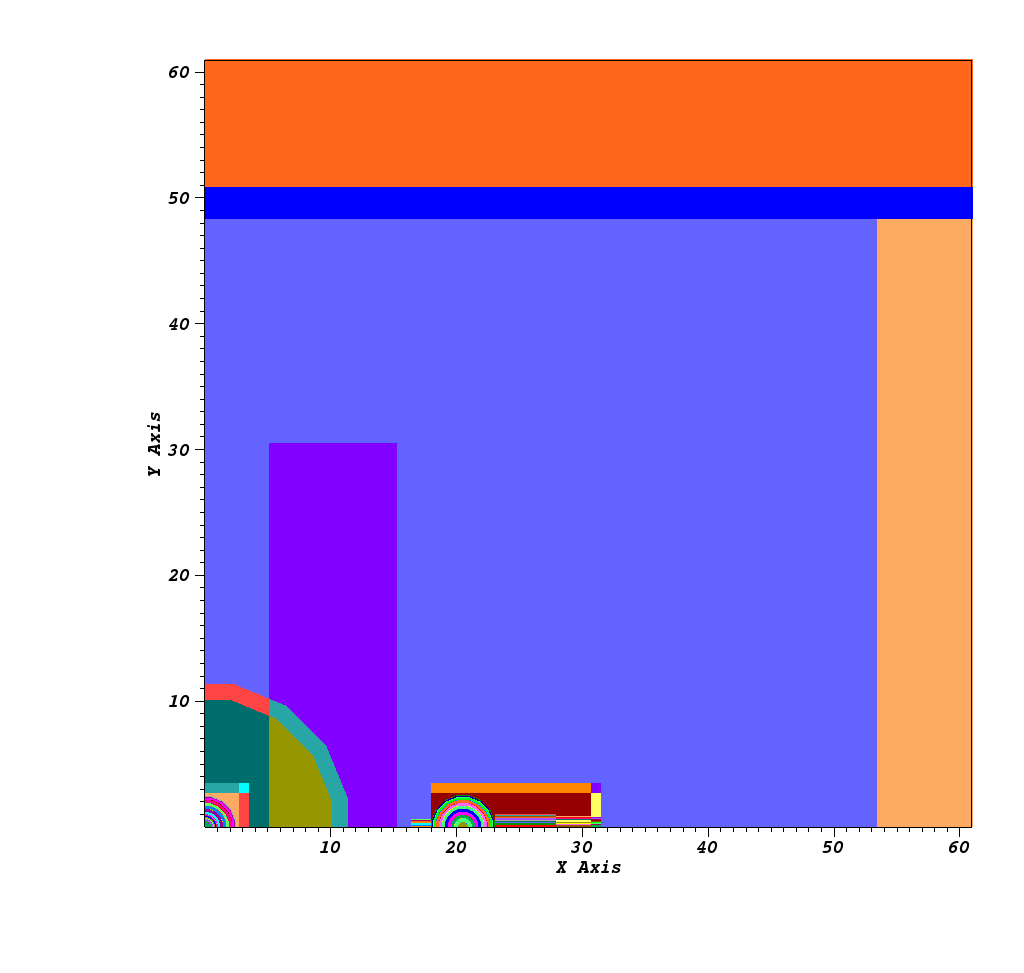
\includegraphics[scale=0.25]{figures/IM12D_val.png}
\end{frame}

\begin{frame}[t]\frametitle{Original Load Balancing, f = 2.63}
\centering
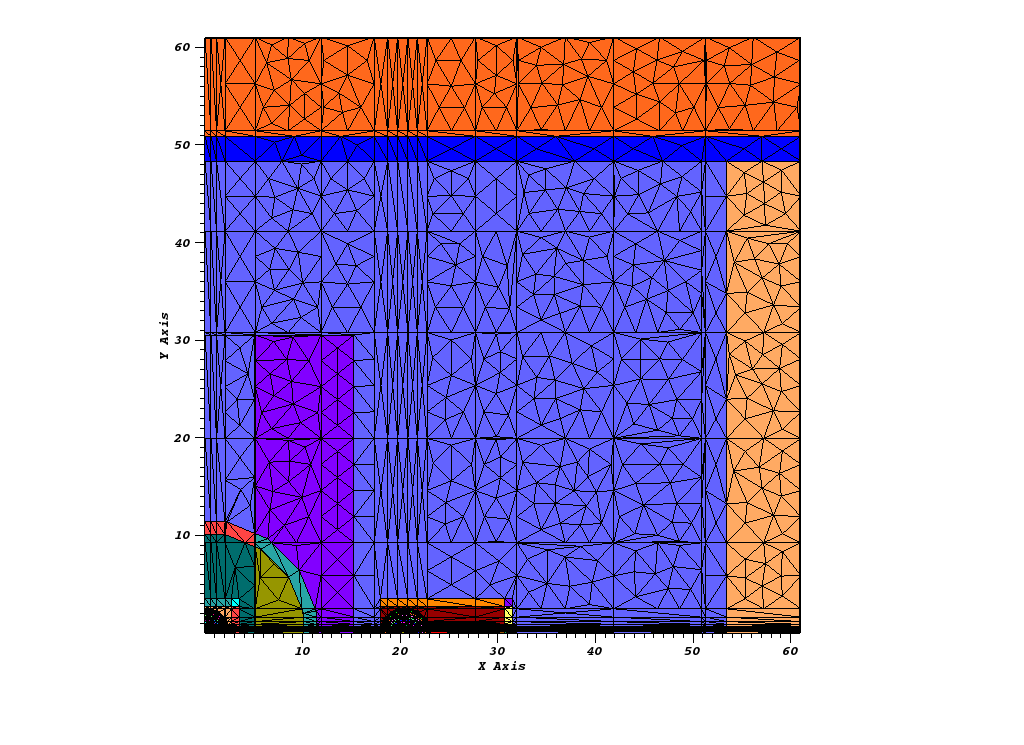
\includegraphics[scale=0.33]{figures/IM1_old_load_balance.png}
\end{frame}

\begin{frame}[t]\frametitle{Load Balancing By Dimension, f = 1.76}
\centering
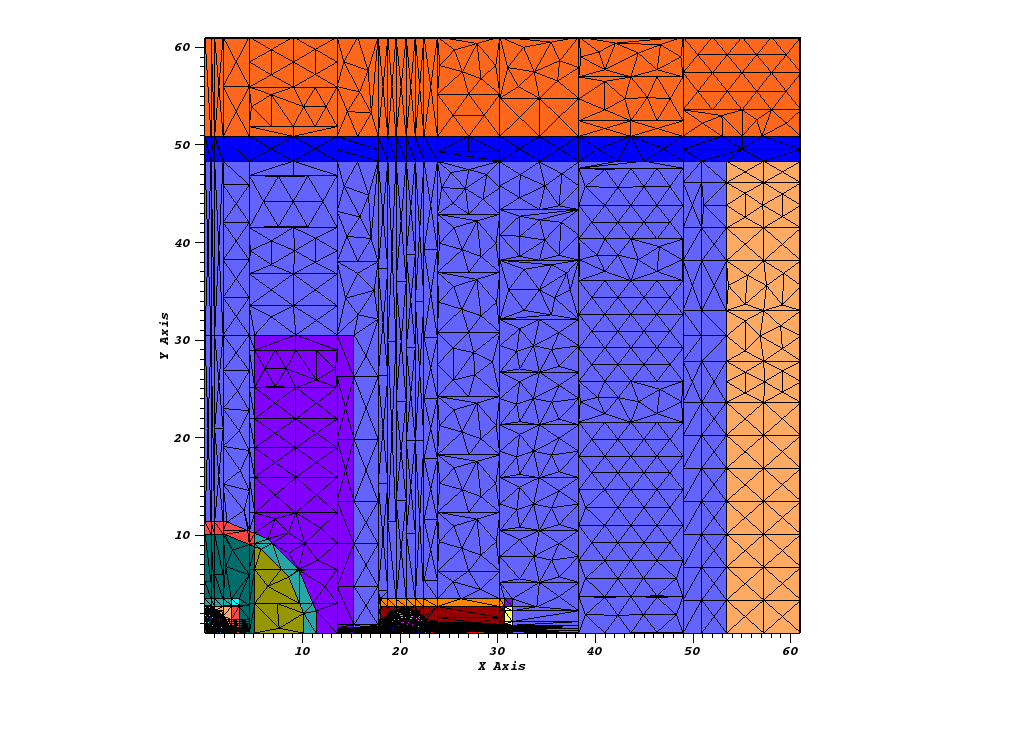
\includegraphics[scale=0.33]{figures/IM1_new_load_balance.png}
\end{frame}

\begin{frame}[t]\frametitle{A closer look}
\centering
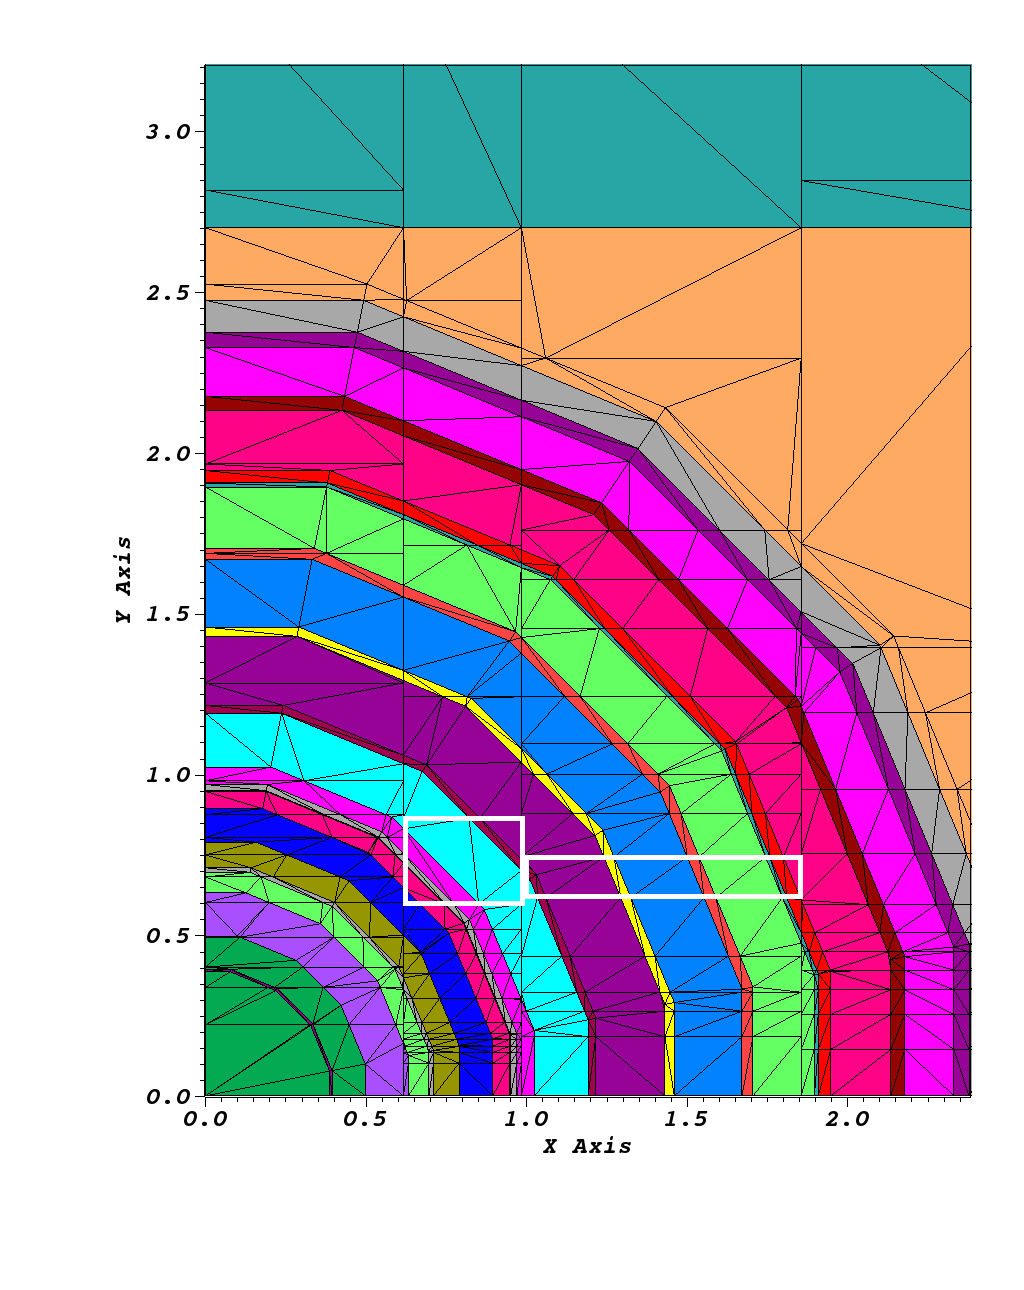
\includegraphics[scale=0.19]{figures/IM1_new_load_balance_zoom.png}
\end{frame}

\section{Conclusions}
%\subsection{}
\begin{frame}[t]\frametitle{Conclusions}
\begin{block}{}
\begin{itemize}
\item The effectiveness of both load balancing algorithms depends on the spatial distribution of fine geometric features, the maximum triangle area used, and the number of subsets the domain is decomposed into.
\item Some improvement is seen for Test Cases 1 and 2.
\item More tinkering with the load balancing by dimension algorithm will be done to study its behavior and potential improvements.
\end{itemize}
\end{block}
\end{frame}

\begin{frame}[t]\frametitle{Future Work - Meshing}
\begin{block}{}
\begin{itemize}
\item Moving away from the Triangle Mesh Generator
	\begin{itemize}
		\item Lack of support
		\item Unable to enforce mesh quality consistently while load balancing problems
	\end{itemize}
\item Spiderweb and heterogeneous grids for 2D and 2D extruded cases.
\item Extrusion based methods that avoid stair stepping.
	\begin{itemize}
		\item Incredibly thin planes in Z that gives the diffusion solver problems.
	\end{itemize}
\item One path forward involves a collaborative effort with Richard Vega (TAMU/Sandia) using a combination of Cubit and OpenFoam.
	\begin{itemize}
		\item Splitting the mesh into subsets rather than the problem geometry
		\item Will allow us to mesh complex 3D problems
	\end{itemize}
\end{itemize}
\end{block}
\end{frame}

\begin{frame}[t]\frametitle{Future Work - Load Balancing}
\begin{block}{}
\begin{itemize}
\item Two more paths for improving the load balancing algorithm have been outlined.
\begin{itemize} 
\item Adaptively splitting the subsets that have large cell counts into smaller subsets, and redistributing subsets amongst processors.
\item Taking advantage of nested parallelism to assign more parallel processes at subsets that require more work to be done.
\end{itemize}
\item Studying the behavior of the communication penalty while load balancing (brought up by Derek Gaston at M\&C 2017).
\item Begin the delevopment of a provably optimal sweep algorithm for ``misaligned'' cellsets.
\end{itemize}
\end{block}
\end{frame}


\begin{frame}[t]\frametitle{Acknowledgments}
\begin{block}{}
A special thank you to the following individuals for their help and support:
\begin{itemize}
\item Drs. Ragusa, Morel, Adams.
\item Michael Adams, Daryl Hawkins, and Dr. Timmie Smith
\item Dr. Andrew Till
\item The CERT team and fellow grad students 
\item Special mention to Rick Vega (TAMU/Sandia) for his help with 3D meshing using OpenFOAM meshing utilities
\item PSAAP-II 
\end{itemize}
\end{block}
\end{frame}

%\begin{frame}[allowframebreaks]{Bibliography}
%\bibliographystyle{alpha}
%\bibliography{science}
% \nocite{*}
%\end{frame}



%\section{\ }
%\begin{frame}[t]\frametitle{Sources}
%	\nocite{Dubcova20111182}
%	\nocite{CHAUVET}
%	\bibliographystyle{ieeetr}
%	\bibliography{science.bib}
%	
%	
%\end{frame}
%



\end{document}